 \documentclass[11pt,a4paper]{article}
\usepackage[utf8]{inputenc}		% LaTeX, comprend les accents !
\usepackage[T1]{fontenc}
\usepackage{natbib}	
%\usepackage[square,sort&compress,sectionbib]{natbib}		% Doit être chargé avant babel      
\usepackage[frenchb,english]{babel}
\usepackage{lmodern}
\usepackage{amsmath,amssymb, amsthm}
\usepackage{a4wide}
\usepackage[capposition=top]{floatrow}
\usepackage{verbatim}
\usepackage{float}
\usepackage{placeins}
\usepackage{flafter}
\usepackage{longtable}
\usepackage{import}
\usepackage{pdflscape}
\usepackage{rotating}
\usepackage{hhline}
\usepackage{multirow}
\usepackage{booktabs}
\usepackage[pdftex,pdfborder={0 0 0},colorlinks=true,linkcolor=blue,urlcolor=blue,citecolor=blue,bookmarksopen=true]{hyperref}
\usepackage{eurosym}
%\usepackage{breakcites}
\usepackage[autostyle]{csquotes}
%\usepackage{datetime}
\usepackage{natbib}
\usepackage{setspace}
\usepackage{lscape}
\usepackage[usenames]{color}
\usepackage{indentfirst}
\usepackage{url}
\usepackage{enumitem}
\usepackage{multirow}
\usepackage{subcaption}
\usepackage[justification=centering]{caption}
\bibliographystyle{agsm}

\usepackage{array}

\newcommand{\isEmbedded}{true}

\graphicspath{{Figures/}}


\begin{document}

\selectlanguage{frenchb}
\title{Statistiques descriptives sortie de grade}

\begin{tabular}{lllr}
	\toprule
	{} & grade 2011 & grade suivant &  n agents \\
	\midrule
	0  &       TTH1 &       TTH2 &  11207 \\
	1  &        &       TTH3 &   4795 \\
	2  &        &       TTM1 &   1047 \\
	3  &        &       TMD1 &    626 \\
	4  &        &        out &    367 \\
	5  &        &       TAJ1 &    363 \\
	6  &        &       TTA1 &    310 \\
	7  &        &       TTT1 &    226 \\
	8  &        &       TTT2 &    194 \\
	9  &        &       TNJ1 &    163 \\
	10 &        &       TPG1 &    141 \\
	11 &        &       TTA2 &    110 \\
	12 &       TTH2 &       TTH3 &   9040 \\
	13 &        &       TTM1 &   1451 \\
	14 &        &        out &    259 \\
	15 &        &       TTA3 &    215 \\
	16 &       TTH3 &       TTH4 &   4893 \\
	17 &        &       TTM1 &   2126 \\
	18 &        &        out &    113 \\
	19 &       TTH4 &       TTM1 &    761 \\
	\bottomrule
\end{tabular}

\begin{center}
	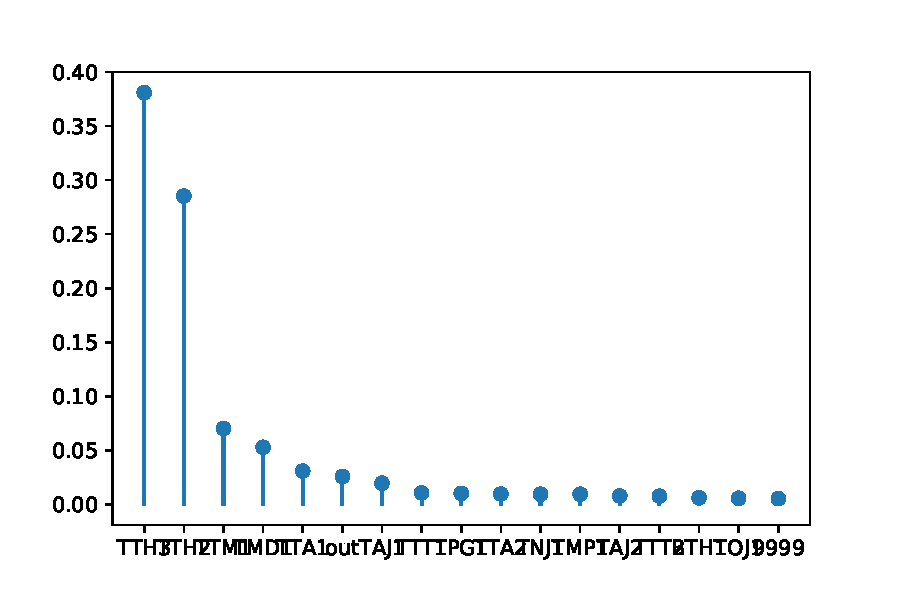
\includegraphics[width=.5\textwidth]{TTH12011.pdf}
	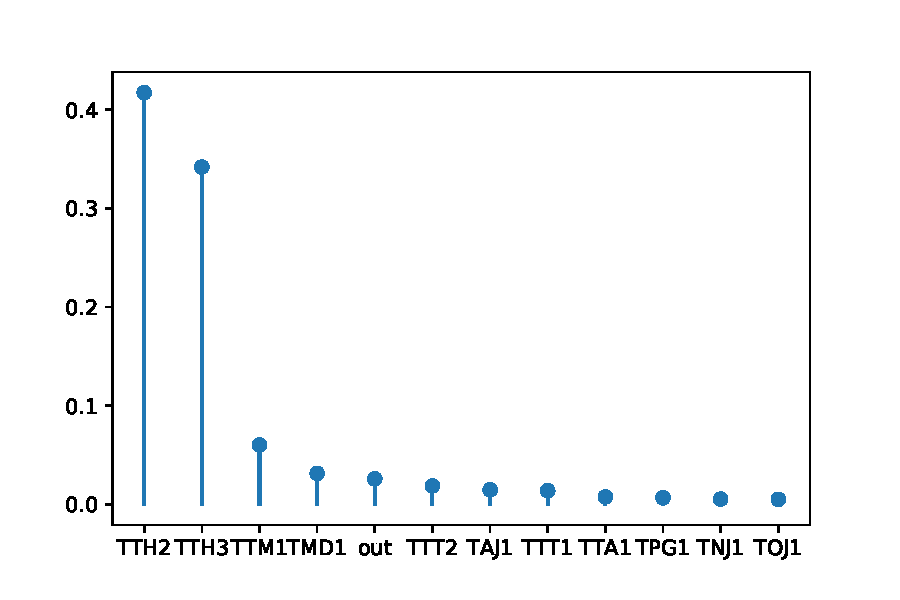
\includegraphics[width=.5\textwidth]{TTH12012.pdf}
	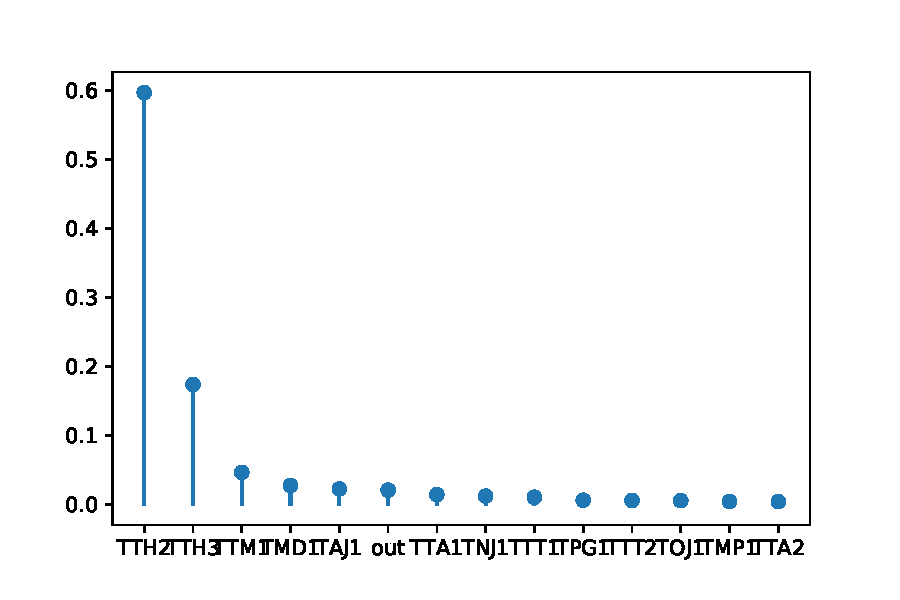
\includegraphics[width=.5\textwidth]{TTH12013.pdf}
	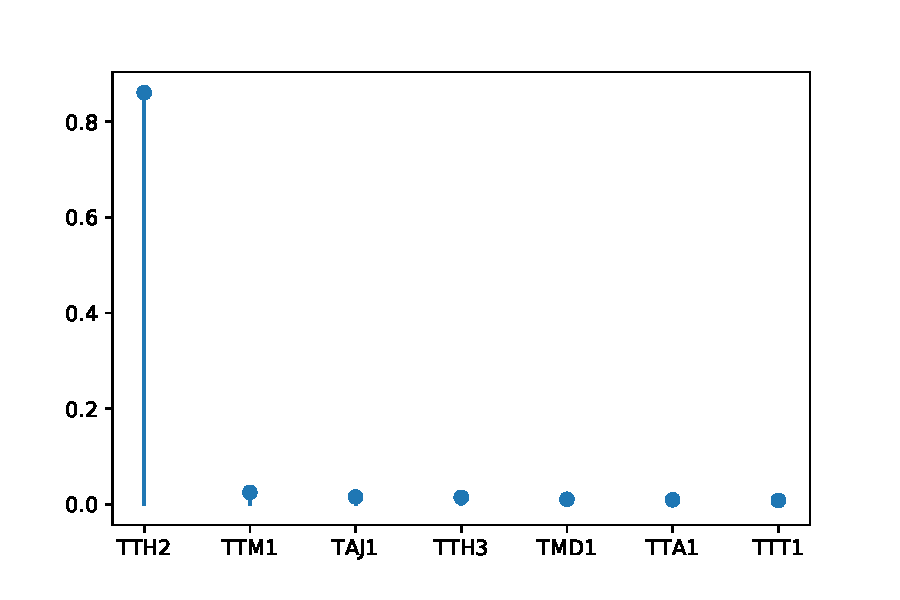
\includegraphics[width=.5\textwidth]{TTH12014.pdf}
\end{center}

\author{}


\maketitle

% Introduction

\end{document}
